\chapter{OPTVM}

O OptVM é um sistema que tem o propósito de dar suporte para a migração de VMs em um ambientes de núvens federadas,
isso é feito através \textit{webservices} utilizando o modelo cliente-servidor, mais específicamente o padrão arquitetural 
Representational State Transfer(REST).

O sistema possui dois principais componentes para atingir seu objetivo: um deles, faz uma filtragem de hosts aplicando 
restrições. E o outro faz uma otimização na escolha de um subconjunto de possíveis hosts para uma VM migrar. 

As restrições que são aplicadas aos possíveis destinos (hosts), elas servem para desconsiderar os destinos 
que não são passiveis de migração por causa de regras de negócio. As restrições no 
OptVM são pré-definidas, ou seja, elas devem ser apenas escolhidas e parametrizadas pelo 
usuário da API, não é possível criar um tipo de restrição. Por exemplo, podem ser definidas regras do tipo: 
uma VM que está localizada em um país, não pode ser migrada para outro país, onde cada país
da regra pode ser parametrizado. Esta regra, pode ser parametrizada com EUA e Israel, por exemplo.
Além disso, as restrições são aplicadas antes da otimização, para o sistema desconsiderar hosts que
não são realmente alvos de migração e limitar o espaço de busca da otimização.

O outro componente, o qual define um melhor subconjunto de hosts faz isso utilizando MOO. Essa
otimização, possui um conjunto de funções objetivo pré-definidas. Esses objetivos também podem ser escolhidos
e parametrizados pelo usuário da aplicação conforme sua necessidade. Os objetivos,
assim como as restrições, são pré-definidos pelo OptVM e o usuário tem a opção de utilizá-los ou não.
Os \textbf{objetivos da otimização}, são interesses do usuário, por exemplo, minimização do consumo de energia.
No OptVM, os objetivos são traduzidos para funções objetivo, do problema de otimização. Ou seja, internamente são tratados
como funções matemáticas que representam o objetivo da otimização.

Como a escolha e parametrização das restrições e funções objetivo da otimização são escolhidos pelo usuário da API,
foi criado um recurso que representa essa configuração e parametrização. Para este recurso foi dado o nome de \textbf{política}. 

O OptVM busca ser uma solução caixa preta, onde, o usuário não necessita saber nada sobre o funcionamento interno, 
algoritmos utilizados, etc. Basta utilizar as \textit{Application Programming Interfaces} (APIs) para fazer uso de suas funcionalidades.
A intenção é que o usuário não precise entender sobre como as coisas são feitas internamente para obter as vantagens do uso do OptVM.

O OptVM é dividido em dois principais componentes: O aplicador de constraints (\textit{constraint applyier})
e o otimizador(\textit{optmizer}). Os dois componentes estão relacionados, porém são representados e 
aplicados separadamente. 

Neste capítulo, serão apresentados aspectos gerais em relação a implementação e uso do OptVM. 
No primeiro momento serão mostrados os dois componentes que integram o sistema. 
Depois disso, técnicas e ferramentas utilizadas, após isso, será demonstrada a ideia do funcionamento 
do serviço e como ele é implementado.

\section{COMUNICAÇÃO}
Em termos gerais, uma API é uma interface de software que pode ser chamada e executada \cite{eizinger}. 

Como o OptVM é um serviço que deve ser disponibilizado para uma arquitetura de 
cliente-servidor de maneira distribuída, haviam três principais maneiras de implementá-lo, 
que eram REST, SOAP e via chamadas RPC. 
Para o desenvolvimento do OptVM foi escolhida a implementação utilizando o modelo REST. 
A escolha desta opção se deu principalmente pelos seguintes motivos:

\begin{enumerate}
\item É um padrão arquitetural maduro;
\item É agnóstico em relação a liguangens de programação;
\item É flexivel em relação ao modelo de comunicação.
\end{enumerate}

Como o padrão arquitetural REST é agnostico em relação ao formato utilizado para fazer a comunicação dos dados. O \textit{econding} 
dos dados pode ser feito da maneira que for mais conveniente para o usuário. No caso do OptVM é possível fazer a comunicação
tanto no formato XML como no formato JSON. O \textit{encoding}
é controlado pelo próprio cliente da aplicação. 
Isso é feito através de cabeçalhos da requisição HTTP.

\section{REPRESENTAÇÃO DO SERVIÇO}

O padrão REST, definido por Fielding \cite{fielding}, sugere que se deve criar uma interface para interação com o sistema. 
Essa interface é representada através de recursos, e a interação com esses recursos é feita através de requisições HTTP, 
as quais contém verbos, o corpo da mensagem, cabeçalhos, entre outras informações. Além disso, o padrão arquitetural também sugere que 
haja links para verificar outras informações e tomar ações sobre os recursos, complementando o HATEOAS.

\subsection{Recursos}

O OptVM trabalha em cima de 2 recursos, chamados políticas(\textit{policies}) e otimizações(\textit{optimizations}). 
Ambos os recursos, trabalham juntos, porém, conseguem trabalhar de maneira independente.

O recurso de políticas é responsável por gerenciar (criar, atualizar, deletar), as políticas
cadastradas. As políticas são compostas por objetivos e restrições. 

Já o recurso das otimizações, é responsável por gerenciar as otimizações executadas pelo sistema. Este recurso,
além de fazer a otimização, também guarda um histórico, com informações mais detalhadas, 
que podem ser consultadas após feitas as otimizações. Além do histórico, o recurso também guarda métricas e informações sobre
a otimização em si, como tempo de execução, número de hosts de entrada/saída, por exemplo.

Conforme REST propõe, são utilizados os verbos para realizar as operações correspondentes
ao que eles se propõe a fazer. Então o verbo POST é utilizado para a criação de recursos,
e o GET para a busca de recurso(s), DELETE para deleção e PUT para atualização.

No geral, as APIs do OptVM estão organizadas da seguinte maneira:

\begin{table}[!htb]
    \centering
    \caption[Recurso Otimização]{Tabela recurso otimização
    \label{tab:tabela-optimization}}
    \begin{tabular}{rrrrr}
        \toprule
            Verbo & URI & Operação \\ 
        \midrule
            GET & \textit{/optimizations} & Todas as otimizações \\
            POST & \textit{/optimizations} &  Cria uma otimização \\
            GET & \textit{/optimizations/:id} & Otimização específica \\
            GET & \textit{/optimizations/:id/details} & Detalhes da otimização \\
            GET & \textit{/optimizations/:id/metrics} & Métricas da otimização \\
        \bottomrule
    \end{tabular}
\end{table}


\begin{table}[!htb]
    \centering
    \caption[Recurso Política]{Tabela recurso policy
    \label{tab:tabela-optimization}}
    \begin{tabular}{rrrrr}
        \toprule
            Verbo & URI & Operação \\ 
        \midrule
            GET & \textit{/policies} & Todas as políticas \\
            POST & \textit{/policies} &  Cria uma política \\
            PUT & \textit{/policies} &  Atualiza uma política \\
            GET & \textit{/policies/:id} & Política específica \\
            DELETE & \textit{/policies/:id} & Exclui específica \\
        \bottomrule
    \end{tabular}
\end{table}



Para cada API, existem campos que fazem parte do corpo da requisição e da resposta
ao criar, buscar e atualizar algum recurso. Alguns campos são representados por entidades e 
podem ter o mesmo formato, tanto na requisição, quanto na resposta, mudando apenas
a obrigatoriedade de alguns atributos da entidade. Isso acontece
com o recurso de \textit{policies} que é representado por uma entidade chamada \textit{Policy}.
Esta entidade tem o seguinte formato:

\begin{table}[!htb]
    \centering
    \caption[resource-optimization-shape]{Tabela propriedades política
    \label{tab:tabela-optimization}}
    \begin{tabular}{rrrrr}
        \toprule
            Nome & Tipo & Descrição \\ 
        \midrule
            \textit{objectives} & Array & Objetivos \\
            \textit{restrictions} & Array &  Restrições \\
        \bottomrule
    \end{tabular}
\end{table}




Como os campos são arrays, eles possuem um conjunto de itens dentro deles. O tipo
de objeto que está dentro do array não é primitivo, e também tem sua representação.
A representação dos tipos de objetos, que são as restrições e os objetivos, são demonstrados
pela Tabela \ref{tab:constraint-shape} e Tabela \ref{tab:objective-shape} respectivamente.

\begin{table}[!htb]
    \centering
    \caption[resource-constraint-shape]{Tabela de propriedades da restrição da política
    \label{tab:constraint-shape}}
    \begin{tabular}{rrr}
        \toprule
            Nome & Tipo & Descrição \\ 
        \midrule
            \textit{type} & Enumeration & Tipo da restrição \\
            \textit{parameters} & Object &  Parâmetros da restrição \\
        \bottomrule
    \end{tabular}
\end{table}

\begin{table}[!htb]
    \centering
    \caption[resource-objective-shape]{Tabela das propriedades do objetivo da política
    \label{tab:objective-shape}}
    \begin{tabular}{rrr}
        \toprule
            Nome & Tipo & Descrição \\ 
        \midrule
            \textit{id} & \textit{enumeration} & Nome do objetivo \\
            \textit{params} & \textit{object} & Parâmetros do objetivo (Opcional) \\
        \bottomrule
    \end{tabular}
\end{table}



A representação da \textit{otimizations} é maior e possui mais subobjetos aninhados
do que a representação do recurso \textit{policies}. Além disso, a otimização utiliza 
um formato em que a requisição e a resposta não possuem o mesmo formato. A requisição
é composta pelo formato das Tabelas \ref{tab:optimization-shape}, \ref{tab:cloud-shape},
\ref{tab:datacenter-shape}, \ref{tab:host-shape} e \ref{tab:vm-shape}:

\begin{table}[!htb]
    \centering
    \caption[Representação de otimização]{Tabela de propriedades da restrição da política
    \label{tab:optimization-shape}}
    \begin{tabular}{rrr}
        \toprule
            Nome & Tipo & Descrição \\ 
        \midrule
            \textit{policyId} & \textit{int} & Identificador da política que deve ser usada \\
            \textit{clouds} & \textit{array} & Lista de núvens da federação \\
        \bottomrule
    \end{tabular}
\end{table}


\begin{table}[!htb]
    \centering
    \caption[Representação da Cloud]{Tabela de propriedades da Nuvem
    \label{tab:cloud-shape}}
    \begin{tabular}{rrr}
        \toprule
            Nome & Tipo & Descrição \\ 
        \midrule
            \textit{id} & \textit{int} & Identificador da nuvem () \\
            \textit{datacenters} & \textit{array} & Lista de datacenters que a nuvem gerencia \\
        \bottomrule
    \end{tabular}
\end{table}
\begin{table}[!htb]
    \centering
    \caption[Representação do Datacenter(DC)]{Tabela de propriedades do Datacenter
    \label{tab:datacenter-shape}}
    \begin{tabular}{rrr}
        \toprule
            Nome & Tipo & Descrição \\ 
        \midrule
            \textit{id} & \textit{int} & Identificador do DC\\
            \textit{name} & \textit{string} & Nome do DC \\
            \textit{localization} & \textit{string} & Localização do DC \\
            \textit{hosts} & \textit{array} & Hosts alocados no DC \\
        \bottomrule
    \end{tabular}
\end{table}



\begin{table}[!htb]
    \centering
    \caption[Representação do Host]{Tabela de propriedades do Host
    \label{tab:constraint-shape}}
    \begin{tabular}{rrr}
        \toprule
            Nome & Tipo & Descrição \\ 
        \midrule
            \textit{id} & \textit{int} & Identificador do Host \\
            \textit{bandwidth} & \textit{int} & Banda larga do Host \\
            \textit{hops} & \textit{int} & Saltos de distância \\
            \textit{requiredMemory} & \textit{int} & Memória requerida por VMs \\
            \textit{hardware} & \textit{object} & Informações de hardware (RAM, \textit{Storage})\\
            \textit{migratingVMs} & \textit{int} & VMs alocadas que estão migrando \\
            \textit{vms} & \textit{array} & VMs alocadas no Host \\
        \bottomrule
    \end{tabular}
\end{table}



\begin{table}[!htb]
    \centering
    \caption[Representação da VM]{Tabela de propriedades da VM
    \label{tab:constraint-shape}}
    \begin{tabular}{rrr}
        \toprule
            Nome & Tipo & Descrição \\ 
        \midrule
            \textit{id} & \textit{int} & Identificador da VM \\
            \textit{ram} & \textit{int} & Memória RAM \\
            \textit{storage} & \textit{int} & Armazenamento \\
            \textit{size} & \textit{int} & Tamanho da imagem \\
            \textit{bandwidth} & \textit{int} & Banda larga \\
            \textit{currentAllocatedMemory} & \textit{int} & Memória RAM alocada \\
            \textit{dirtyPages} & \textit{int} & Páginas sujas \\
        \bottomrule
    \end{tabular}
\end{table}




A resposta, utiliza somente os identificadores das entidades envolvidas. Não
é utilizado a representação completa dos hosts, sendo assim, é possível
diminuir o corpo da mensagem. Porém, caso o usuário da API queira obter 
o corpo completo dos itens selecionados, basta que ele utilize a chamada de 
detalhes do recurso \textit{optimizations}. Para a resposta o formato das
tabelas \ref{tab:response-shape} e \ref{tab:response-host}:

\begin{table}[!htb]
    \centering
    \caption[response-optimization-shape]{Tabela das propriedades da resposta
    \label{tab:tabela-optimization}}
    \begin{tabular}{rrrrr}
        \toprule
            Nome & Tipo & Descrição \\ 
        \midrule
            \textit{id} & \textit{int} & Identificador da resposta \\
            \textit{hosts} & \textit{array} & Melhores hosts\\
            \textit{metric} & \textit{string} & Link para as métricas da otimização \\
            \textit{details} & \textit{string} & Link para informações mais detalhadas da otimização \\
        \bottomrule
    \end{tabular}
\end{table}


\begin{table}[!htb]
    \centering
    \caption[response-optimization-shape]{Tabela das propriedades da resposta
    \label{tab:tabela-optimization}}
    \begin{tabular}{rrrrr}
        \toprule
            Nome & Tipo & Descrição \\ 
        \midrule
            \textit{cloud} & \textit{int} & Identificador da núvem \\
            \textit{datacenter} & \textit{int} & Identificador do datacenter \\
            \textit{host} & \textit{int} & Identificador do host \\
        \bottomrule
    \end{tabular}
\end{table}


\section{APLICADOR DE CONSTRAINTS (CONSTRAINT APPLYIER)}

Como citado na introdução do capítulo, o OptVM utiliza restrições pré-definidddas.
Para o entendimento de como funciona as o aplicador de restrições, é importante conhecer os tipos de 
restrições e como elas funcionam.

\subsection{Tipos de restrições (constraints)}

As restrições pré definidas, tem um \textit{alias} para que o usuário do serviço faça a identificação no uso delas.
Os tipos de restrições disponibilizadas pelo OptVM operam em 3 níveis, são eles: \textbf{cloud}, \textbf{datacenter} (DC)
e \textbf{hosts}.

Cada restrição tem uma responsabilidade específica, uma regra de negócio que não deve ser infringida. 
As restrições disponibilizadas e seus respectivos níveis são as seguintes:

\begin{enumerate}
  \item Cloud:
  \begin{enumerate}
    \item \textit{CloudName}: Nome de uma nuvem em que o host não pode ser alocado.
  \end{enumerate}

  \item DC:
  \begin{enumerate}
    \item \textit{Conflito}: Pode conflitar uma localização, por exemplo, uma VM dos USA, não pode habitar em um host de ISRAEL;
    \item \textit{Custo}: Os custos que irão gerar ultrapassam os parâmetros.
  \end{enumerate}

 \item Host
  \begin{enumerate}
    \item \textit{Dependência}: Depende que o host tenha um sistema operacional(OS) ou hypervisor específico (baseado em seus parâmetros);
    \item \textit{Coabitação}: Dependendo dos parâmetros da constraints, exige que o host seja vizinho (1 hop de distância).
  \end{enumerate}
  
\end{enumerate}

\subsection{Algoritmo}
O \textit{constraint applyier} tem a responsabilidade de remover os hosts que não atendem à
uma ou mais restrições estabelecidas pelo usuário. Como as restrições operam nos 3 níveis,
é importante que algoritmo tenha acesso a um contexto onde obtenha informações sobre as núvens, 
datacenters e hosts disponíveis.

O algoritmo que aplica as constraints, consiste em iterar sobre as constraints ordenadas da mais significativa 
(operam em nível de cloud), para a menos significativa (operam em nível de host), e remover os itens que não atendem as
restrições, após cada iteração.

O pseudocódigo do algoritmo é representado da seguinte maneira:

\begin{algorithm}
    \caption{Constraint Applyier}
    \KwIn{as $constraints$ restrições, $context(Clouds, DCs, Hosts)$ contexto com todas as opções disponíveis}
    \KwOut{$context'(Clouds, DCs, Hosts)$ somente com Clouds/DCs/Hosts que atendem as restrições} 

    $context'\leftarrow context$\\
    \For {$constraints \in constraints$} {
        \If {$c$ é do tipo CLOUD} {
            aplica a $constraints$ nas núvens do contexto\\
            $context'\leftarrow nuvensAtualizadas$\\
        }
        \ElseIf {$constraints$ é do tipo DC} {
            aplica a $constraints$ nas DCs do contexto\\
            $context'\leftarrow datacentersAtualizados$\\
        }
        \ElseIf {$constraints$ é do tipo HOST} {
            aplica a $constraints$ nas Hosts do contexto\\
            $context'\leftarrow hostsAtualizados$\\
        }
    }

\end{algorithm}



A intenção de aplicar as restrições ordenadas das mais significativas, que são as 
entidades que eliminarão mais destinos de uma vez (\textit{Clouds} e \textit{Datacenters}),
para as menos significativas (\textit{Hosts}), para que diminua o número de iterações.
Pois quando, por exemplo, um \textit{datacenter} não atende uma restrição, nenhum host daquele datacenter 
são elegíveis como um possível destino, então, as restrições em nível de host para
os hosts desse determinado datacenter nem devem ser executadas. 

Uma representação visual, de como o algoritmo funcionaria, pode ser vista na Figura \ref{fig:constraintapplyier}. 
A ideia é que funcione semelhante a uma estrutura de árvore com três níveis, e que quando um nó pai não atende 
a uma restrição, consequentemente a sub-árvore também não atende. E a avaliação é feita top-down, começando pela
raiz e indo em direção aos nós folhas.

\begin{figure}[!htb]
  \centering
  \caption{Exemplo de aplicação das constraints}
  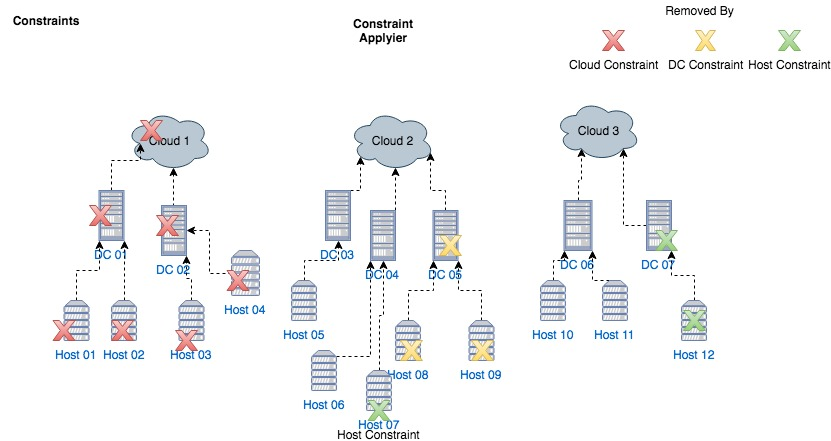
\includegraphics[width=1\textwidth]{./dados/figuras/constraintapplyier}
  \label{fig:constraintapplyier}
\end{figure}

A Figura \ref{fig:constraintapplyier} mostra como as constraints aplicadas em seus respectivos níveis, eliminariam a possíbilidade
da VM migrar para determinado host. Na Figura \ref{fig:constraintapplyier}, foram representados os seguintes casos:

\begin{enumerate}
\item A \textbf{Cloud 1} não atende à alguma restrição escolhida em nível de nuvem, então nenhum de seus DCs e por consequência hosts dos DCs, serão alvos válidos;
\item O \textbf{Datacenter 05} não atende alguma restrição em nível de DC, então nenhum de seus hosts estarão disponíveis como alvo de migração;
\item E os \textbf{Host 07 e Host 12} não atendem alguma restrição em nível de host;
\item Um caso mais específico é quando o \textbf{Host 12} não atende a alguma restrição, logo o \textbf{DC 07} não terá nenhum host válido, então também deve ser desconsiderado.
\end{enumerate}

\section{OTIMIZADOR (OPTIMIZER)}

Considerando que o cliente da API é uma federação de nuvens computacionais.
O \textit{optimizer} é responsável por otimizar a seleção dos hosts disponíveis nas nuvens da federação,
para a VM que necessita migrar. O objetivo é alcançar um melhor subconjunto para a alocação da VM. 
Além disso, a seleção desse subconjunto é selecionado atendendo os objetivos e restrições da \textbf{política} 
selecionada para a otimização, escolhida pelo usuário.

A otimização feita no OptVM faz uso de GAs. Os GAs fazem iterações sobre 
uma população que é iniciada aleatoriamente no algoritmo. Para cada iteração,
o algoritmo avalia os indivíduos ou soluções da população pela \textit{fitness function}, 
que também é chamada de função objetivo. Após a avaliação dos indivíduos, é
feita a seleção dos melhores avaliados e também é feito o crossover, gerando uma nova população,
que é mais evoluida e mais adequada ao problema. O número de iterações
feitas é escolhido pelo usuário do algoritmo. Quanto mais iterações houver, mais evoluida
estará a população, porém, maior será o consumo computacional. Caso o número de iterações
for muito alto, pode inviabilizar o uso do algoritmo por causa do tempo de resposta.

No OptVM, os objetivos são dinâmicos, ou seja, é possível que o usuário da API escolha por alguns
objetivos e não por outros. Os objetivos disponíveis no OptVM são três, dos quais uma combinação de
dois ou os três podem ser escolhidos, são eles:

\begin{enumerate}
\item Minimização do consumo de energia;
\item Minimização do tempo de instalação;
\item Minimização da sobrecarga da migração.
\end{enumerate}

Como a otimização possui um conjunto de indivíduos, que formam uma população, cada indivíduo
da população representa uma possível solução para o problema.  Nos algoritmos de 
otimização o indivíduo possui uma representação (\textit{encoding}), que pode ser feita
de diversas maneiras, de maneira binária, por inteiros, entre outros tipos de representação.

Como uma representação representa uma solução para o problema, no OptVM, a 
representação escolhida foi uma representação de inteiros, ou seja, uma solução
para o problema é um array de inteiros com tamanho do subconjunto escolhido pelo
usuário onde cada número representa um host. Os números contidos no subconjunto
representam o indice de um host de todos os disponíveis.

\[
  Solution=
  \left[{\begin{array}{cccccc}
    36 & 5 & 120 \\
  \end{array}}\right
  ]
\]

No exemplo, o tamanho escolhido para o subconjunto é de 3 hosts, ou seja, 
a otimização busca achar o melhor subconjunto de 3 hosts dentre os N disponíveis. 
No exemplo, os 3 hosts escolhidos na solução, são os hosts 36, 5 e 120 do conjunto de N hosts.

\section{FUNÇÕES OBJETIVO (OFs)}
Como citado na seção anterior, são disponibilizadas três OFs e que internamente, o OptVM
utiliza funções matemáticas para a representação das OFs. Nesta seção será demonstradas e
explicadas as funções utilizadas pelo OptVM.

As funções objetivo, assim como as restrições, utilizam a representação das entidades 
(host, vm) e seus atributos para fazer o processamento necessário na etapa em que é responsável.

\subsection{Minimização do consumo de energia}
O consumo de energia é um aspecto importante a ser minimizado quando
se trata da migração de uma VM. No contexto da otimização da seleção 
de hosts para fazer a migração de uma VM, o host a ser buscado
para receber a VM, deve ser o que impacte menos em relação ao consumo de 
energia no processo de migração da VM.

Segundo \cite{beloglazov}, o consumo de energia dos \textit{hosts} está relacionado
ao uso de recursos de CPU. Apesar de estar relacionado, outros aspectos devem ser levados
em conta, como a capacidade do CPU. A mesma utilização de CPU em processadores de capacidades
diferentes, implica que o processador de menos capacidade gaste mais energia que o de maior capacidade.

Conforme \cite{beloglazov} existe uma relação entre o consumo de CPU e o gasto de energia. Sendo assim,
uma importante variável para esta OF é a utilização de CPU. O valor atribuído à utilização de CPU na OF é uma 
percentagem, e é representada por $ U\textsubscript{cpu}_i $ na Equação \ref{eq:energ}. 

Além disso, duas outras variáveis são utilizadas para calcular a energia gasta pelo \textit{host}, que são:
O máximo de energia suportado pelo host e o mínimo (quando ele se encontra em estado inativo). Estas outras duas
medidas são representadas por $ host_i $ $ (p\textsubscript{max}_i) $ e $ host_i $ $ (p\textsubscript{min}_i) $
respectivamente.

Com isso, podemos definir que a Equação que representa o consumo de energia é a seguinte:

\begin{equation}
energ(h_i ) =  ((p\textsubscript{max}_i - p\textsubscript{min}_i) * U\textsubscript{cpu}_i + p\textsubscript{min}_i) 
\label{eq:energ}
\end{equation}

\subsection{Minimização do tempo de instalação}

Para a migração de uma VM occorer, algumas etapas devem ser concluídas, são elas: 
a detecção de uma migração, a transferência da VM para o \textit{host} de destino 
e a instalação no mesmo. Esta OF está interessada em escolher um \textit{host} que 
sobrecarregue o mínimo possível a última etapa da migração. Uma VM pode ser considerada
instalada no host de destino, quando ela estiver configurada e pronta para continuar o seu
uso. Esta medida, neste trabalho, é chamada de Tempo de Reconfiguração ($ t\textsubscript{reconf} $).

Outra medida que está ligada ao tempo de reconfiguração é a capacidade do host. Esta 
medida é dada pelo produto do número de núcleos de processamento pelo MIPS (Milhares de
instruções por segundo). Esta medida pode ser observada na Equação \ref{eq:cap}:

cap:
\begin{equation}
\begin{split}
cap\textsubscript{h}_i = \sum_{k=1}^{Npes}(pe_k * mips_k)
\end{split}
\label{eq:cap}
\end{equation}

O tempo de fixação de uma VM no destino é obtido através da quantidade de memória 
já alocada para as VMs do host de destino $\sum_{j=1,i \neq j}^{N} M_j$ dividido pela
largura de banda do host $larg\textsubscript{ban}({h}\textsubscript{i})$. Estas variáveis 
são utilizadas por interferirem diretamente no tempo de fixação da VM.
Sendo assim a Equação \ref{eq:tfix} descreve o tempo de fixação.

\begin{equation}
t\textsubscript{fix}\textsubscript{(vm}_i\textsubscript{)} = \sum_{j=1,i \neq j}^{N} M_j/larg\textsubscript{ban}({h}\textsubscript{i})
\label{eq:tfix} 
\end{equation}

Com hipervisores como \textit{Xen} e \textit{VMWare} é possível fazer migração a quente.
Para este tipo de migração ocorrer, é necessário que as páginas sujas da VM sejam transferidas.
Para isso acontecer, é necessário que haja um certo número de iterações e essas iterações deduzem
o número de páginas sujas da VM. Sendo assim, tanto o número de iterações ($ iter $)
quanto a quantidade de páginas sujas ($ v\textsubscript{dr} $) são significativos para 
o tempo de reconfiguração. Sendo assim, a equação \ref{eq:reconf} representa a OF 
de tempo de reconfiguração.

\begin{equation}
\begin{split}
t\textsubscript{reconf}\textsubscript{(vm}_i\textsubscript{)} = \dfrac{ (v\textsubscript{dr}(vm_i) * iter) + M_i}{larg\textsubscript{ban}} \; + t\textsubscript{fix}\textsubscript{(vm}_i\textsubscript{)} \\
0<i<N, N <= Cap\textsubscript{hosts}
\end{split}
\label{eq:reconf}
\end{equation}

\subsection{Minimização da sobrecarga da migração}

Segundo \cite{anand}, para minimizar o tráfego que uma migração gera 
é necessário diminuir a quantidade de dados a ser transferida. Porém,
quantificar a sobrecarga da migração é uma operação complexa por conta 
das diferentes variáveis que um \textit{host} tem. Para resolver este problema 
\cite{anand} identificaram que uma solução é atribuir pesos para recursos do 
host, atribuindo um peso maior para os recursos que são considerados mais impactantes
na sobrecarga e menor para menos impactantes. Esses pesos são distribuidos 
da seguinte maneira: 0,8 para banda larga; 0,6 para armazenamento; 0,4 para a memória 
e 0,1 para o CPU.

\begin{equation}
sob\textsubscript{mig}(h_i) = \sum_{i=1}^{m}r_i * w_i
\label{eq:sobHi}
\end{equation}

Como diferentes \textit{hosts} participam da migração, todos os 
\textit{hosts} devem ser considerados na equação \ref{eq:sobrecarga} de 
sobrecarga da migração. No OptVM, para efeito de simplicidade, foi considerado
que somente o host de origem e host de destino estão envolvidos na migração.

\begin{equation}
\begin{split}
sob\textsubscript{mig} = \sum_{i=1}^{N}sob\textsubscript{mig}(h_i) * P  \\
N <= Cap\textsubscript{hosts}
\end{split}
\label{eq:sobrecarga}
\end{equation}

\section{FUNCIONAMENTO DO SERVIÇO}

A utilização do serviço, sugere que seja seguido um fluxo. Não é obrigatório
utilizar este fluxo. Porém o OptVM é utilizado em sua totalidade se o seguir. 
O próprio serviço ajuda o usuário seguir o fluxo, através do HATEOAS, indicando 
links e próximas ações e consultas que podem ser feitas pelo consumidor da aplicação.

A ideia é que no caso de uso mais simples de utilização do serviço, 
para fazer uma otimização, é seguido o seguinte fluxo:

\begin{enumerate}
 \item Criação de uma política, com seus objetivos e restrições de negócios;
 \item Envio do conjunto de núvens/DCs/Hosts para ser feita a otimização;
 \item Obtenção do subconjunto de hosts otimização.
\end{enumerate}

\begin{figure}[!htb]
  \centering
  \caption{Exemplo de aplicação das constraints}
  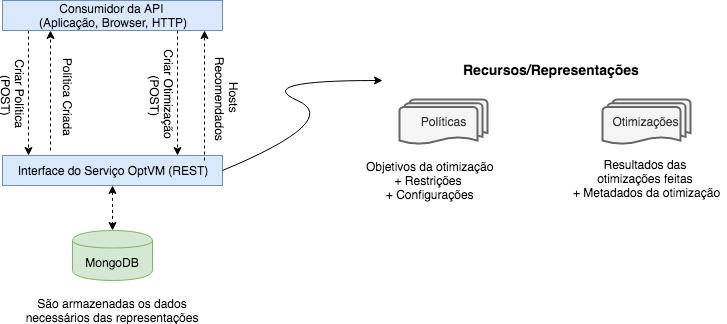
\includegraphics[width=1\textwidth]{./dados/figuras/overview.png}
  \label{fig:overview}
\end{figure}

Apesar do caso de uso básico, é possível utilizar a API de maneiras diferentes,
e fazer as combinações que forem mais úteis para o usuário. Por exemplo, é possível
criar uma otimização sem uma política, para este caso, serão adotados valores
padrões para os parâmetros obrigatórios da política e todos os objetivos na otimização.

A criação de uma política, é feita enviando os objetivos e as restrições.
Após criada a política, a mesma pode ser utilizada em uma otimização. Para a 
criação da política, pode ser utilizado o seguinte formato:

\begin{lstlisting}[language=json,firstnumber=1]
{
  "objectives": ["MIN_ENERGY_CONSUMPTION", "MIN_INSTALLATION_TIME"],
  "constraints": [
    {
      "type": "Cost",
      "params": {
        "max_per_memory": 0.35
      }
    }
  ]
}
\end{lstlisting}

Após a criação de um política, é possível usá-la para fazer otimizações. A mesma
política, pode ser utilizada por múltiplas otimizações.

A criação de uma otimização, retorna um objeto com um resumo dos melhores hosts
e sua identificação, para melhorar o destino da VM.
Além disso, é possível obter detalhes de execução, através de \textit{/metrics}, assim
como detalhes da otimização através da URI \textit{/details}.

No exemplo, a criação de um recurso de otimização deve-se ser utilizado o seguinte formato, 
para o corpo da requisição. Está sendo utilizado o formato JSON, porém, o mesmo se aplica 
também para o XML:



\begin{lstlisting}[language=json,firstnumber=1]
{
  "id": 1,
  "policyId": 2,
  "clouds": [
    {
      "id": 1,
      "name": "Test",
      "datacenters": [
        {
          "id": 1,
          "hosts": [
            {
              "id": 1,
              "vms": [{"id": 10}]
            },
            ...
          ]
        },
        ...
      ]
      ...
    }
  ]
}
\end{lstlisting}

Quando o OptVM recebe uma requisição de otimização, o fluxo da figura \ref{fig:fluxograma-otimizacao}
é seguido para processar a requisição e retornar as melhores opções de seleção de host
para o usuário.

\begin{figure}[!htb]
  \centering
  \caption{Exemplo de aplicação das constraints}
  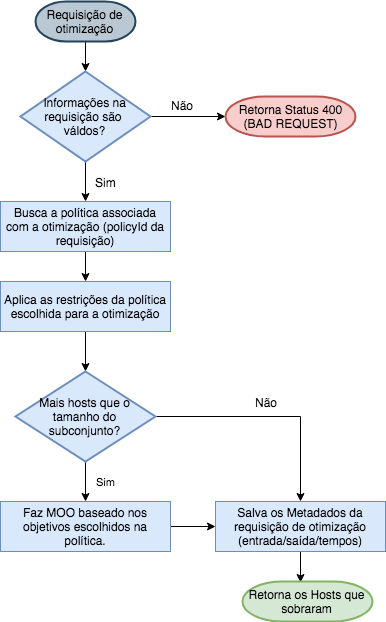
\includegraphics[width=0.5\textwidth]{./dados/figuras/fluxograma-otimizacao.png}
  \label{fig:fluxograma-otimizacao}
\end{figure}

E a resposta tem o seguinte formato:

\begin{lstlisting}[language=json,firstnumber=1]
{
  "id": 1,
  "policyId": 2,
  "hosts": [
    "option_1": [
      {
        "cloud": 1,
        "datacenter": 2,
        "host": 1
      },
      ...
    ] 
    ...
  ],
  "policy": "http://host.domain/api/policies/2",
  "metrics": "http://host.domain/optimizations/1/metrics"
}
\end{lstlisting}

Apesar do exemplo estar mostrando arrays com apenas um item,
tanto para a requisição como para a resposta, muito provavelmente 
haverá outras opções. Cada opção contém um subconjunto com o tamanho
N escolhido pelo usuário da API. 

\section{TECNOLOGIAS UTILIZADAS}

O desenvolvimento de uma API pode envolver ferramentas como bibliotecas, frameworks e 
bancos de dados. Nesta seção, são apresentadas as principais ferramentas que foram utilizadas para
fazer o desenvolvimento da API. 

\subsection{MOEA Framework}
Segundo \cite{moea}, o \textit{Moea Framework} é um framework é uma
biblioteca gratuita que serve para experiementar e desenvolver
algoritmos evolucionários baseados em múltiplos objetivos. Nesta biblioteca
existem diversos algoritmos, incluindo vários tipos de GAs, que foram utilizados
no desenvolvimento deste trabalho.

\subsection{MongoDB}
MongoDB é um banco de dados orientado a documentos. A escolha dele foi
feita por dois principais motivos:

\begin{enumerate}
  \item Facilidade no desenvolvimento;
  \item Facilidade de armazenamento de dados não estruturados.
\end{enumerate}

O mongoDB faz o armazenamento dos documentos, que, basicamente são um JSON
armazenado de maneira binária e eficaz. O banco separa esses JSONs em coleções,
que podem ser separadas da maneira que o usuário achar melhor.

Como o MongoDB é orientado a documentos, é possível utilizá-lo para armazenar
dados que não necessáriamente sigam a mesma estrutura sempre. Isso é importante no contexto do
OptVM por causa da flexibilidade que o próprio OptVM permite. Por exemplo, no
caso das restrições, o OptVM permite que sejam criadas restrições de diversos tipos,
tendo parâmetros também de tipos diferentes, sendo assim, utilizar um banco de 
dados não estruturado, é uma alternativa melhor, pois permite flexibilidade no armazenamento
dos itens.
